\section{Introduction}
\label{sec:intro}

Large Language Model (LLM)-driven evolutionary code search has rapidly emerged as a promising paradigm for automated scientific and engineering discovery. In this setting, LLMs propose program mutations within search loops that are guided by executable feedback \citep{romera-paredes2024,novikov2025c,georgiev2025c,lange2025b,assumpcao2026,cemri2026,liu2026}.
This paradigm has produced strong results across mathematical construction, systems optimization, algorithm design, and GPU kernel engineering, including improved bounds for combinatorial problems, better packing constructions, compiler and scheduling heuristics \citep{romera-paredes2024,novikov2025c,georgiev2025c,cheng2025b,guo2025,cao2026,wiedemann2026}.
In this study, we define an \textbf{evolutionary coding agent} as a system with a task specification and executable evaluator, a population or archive of candidate programs, one or more LLMs that generate code mutations, recombinations, or refinements, and a search procedure that selects which programs and contexts feed future generations. A \textbf{search trace} is the full record produced by such a system: generated programs, scores, execution feedback, parent-child relations, prompts, model choices, and intermediate artifacts.

\begin{figure}[t]
    \centering
    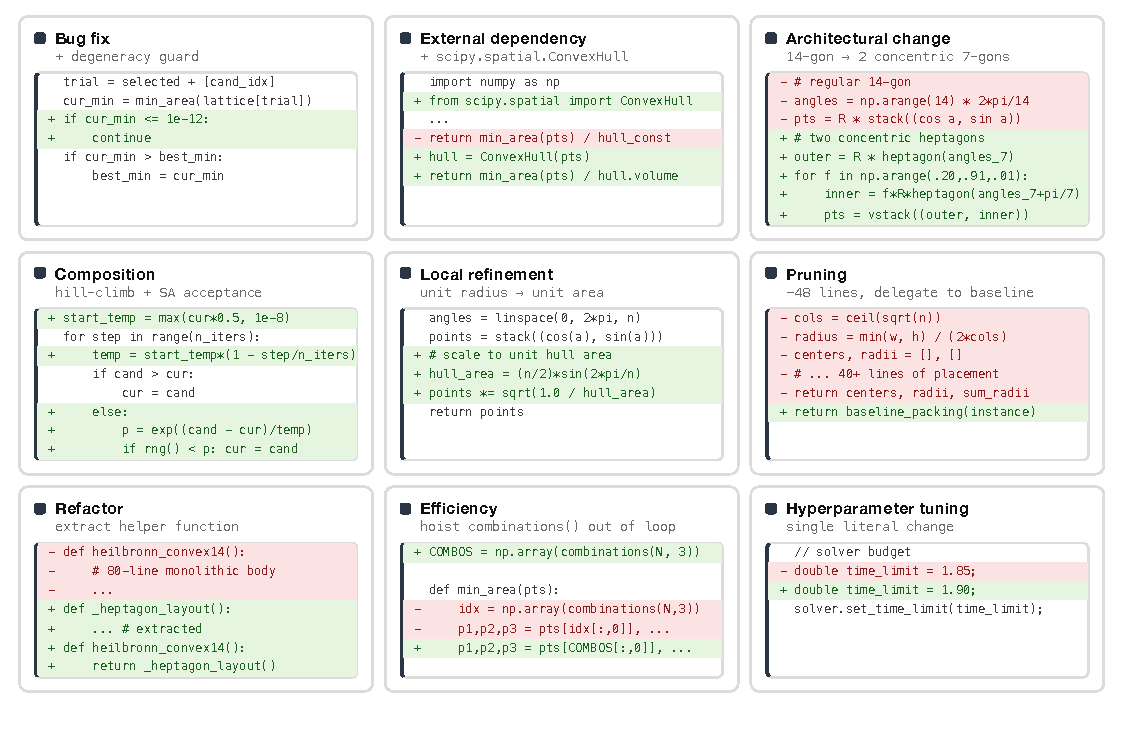
\includegraphics[width=\linewidth]{Figures/evolutionary_edits_taxonomy.pdf}
    \caption{\textbf{A taxonomy of edits performed by evolutionary coding agents.} Each panel shows a representative parent--child diff (added lines in green, deleted lines in red) drawn from EvoTrace runs and labeled with one of nine recurring categories: \emph{Bug fix}, \emph{External dependency}, \emph{Architectural change}, \emph{Composition}, \emph{Local refinement}, \emph{Pruning}, \emph{Refactor}, \emph{Efficiency}, and \emph{Hyperparameter tuning}. The categories range from minimal numeric edits (a single literal change) to structural rewrites (replacing a 14-gon with two concentric heptagons), and they form the basis of the LLM-as-judge edit annotation used throughout the paper. Edits are typically multi-label; we examine prevalence and per-edit utility in \S\ref{sec:static-analysis}.}
    \label{fig:evolutionary_edits_taxonomy}
\end{figure}

Despite rapid interest and empirical progress, the internal dynamics of evolutionary coding agents remain poorly understood. Existing work often reports final best scores, aggregate success rates, or a handful of illustrative trajectories, but such endpoints obscure the pathways and mechanisms by which improvements arise. While evolutionary coding agents sometimes demonstrate clear advantages over baselines such as independent sampling, greedy refinement, or beam-style search, these gains are highly sensitive to choices in task design, initialization, evaluator specification, or model configuration.
There is consequently no clear consensus on what these systems are actually evolving: whether progress comes from discovering new program structure, tuning parameters of already-known strategies, recombining concepts already present in the model, or preserving early biases in the population.
This motivates the central question we address: \textit{What do evolutionary coding agents evolve, and how do their search dynamics produce improvements?}

To address this question, we introduce a dataset of evolutionary coding traces collected across multiple frameworks, models, and task families, covering mathematical constructions and algorithmic programming tasks. Rather than treating each run only by its final score, we study the full trajectory of generated programs: which solutions are explored, which lineages produce major improvements, and how stable those improvements are. The resulting dataset is intended to make evolutionary coding agents analyzable as dynamic systems, not just benchmark submissions.

Analyzing these traces is non-trivial: a single run may generate hundreds of unique programs, and each candidate can differ from its ancestors through non-local structural changes, small numerical edits, prompt-driven rewrites, or evaluator-specific hacks. To make runs comparable, we develop a unified trace representation together with an annotation and measurement pipeline. The representation exposes the search graph, candidate programs, evaluations, and lineage information, enabling analyses of population structure, diversity, best-lineage stability, counterfactual model or context changes, and the decomposition of structural versus parametric gains.



We use this framework as a diagnostic tool for understanding both progress and failure in evolutionary coding.
Our analysis covers four diagnostics: static measures of program complexity and lineage utilization (\S\ref{sec:static-analysis}), deterministic detection of cycling, the re-introduction of previously-deleted lines (\S\ref{sec:cycling}), 
\begin{wrapfigure}{r}{0.65\textwidth}
    \centering
    \vspace{-0.8em}
    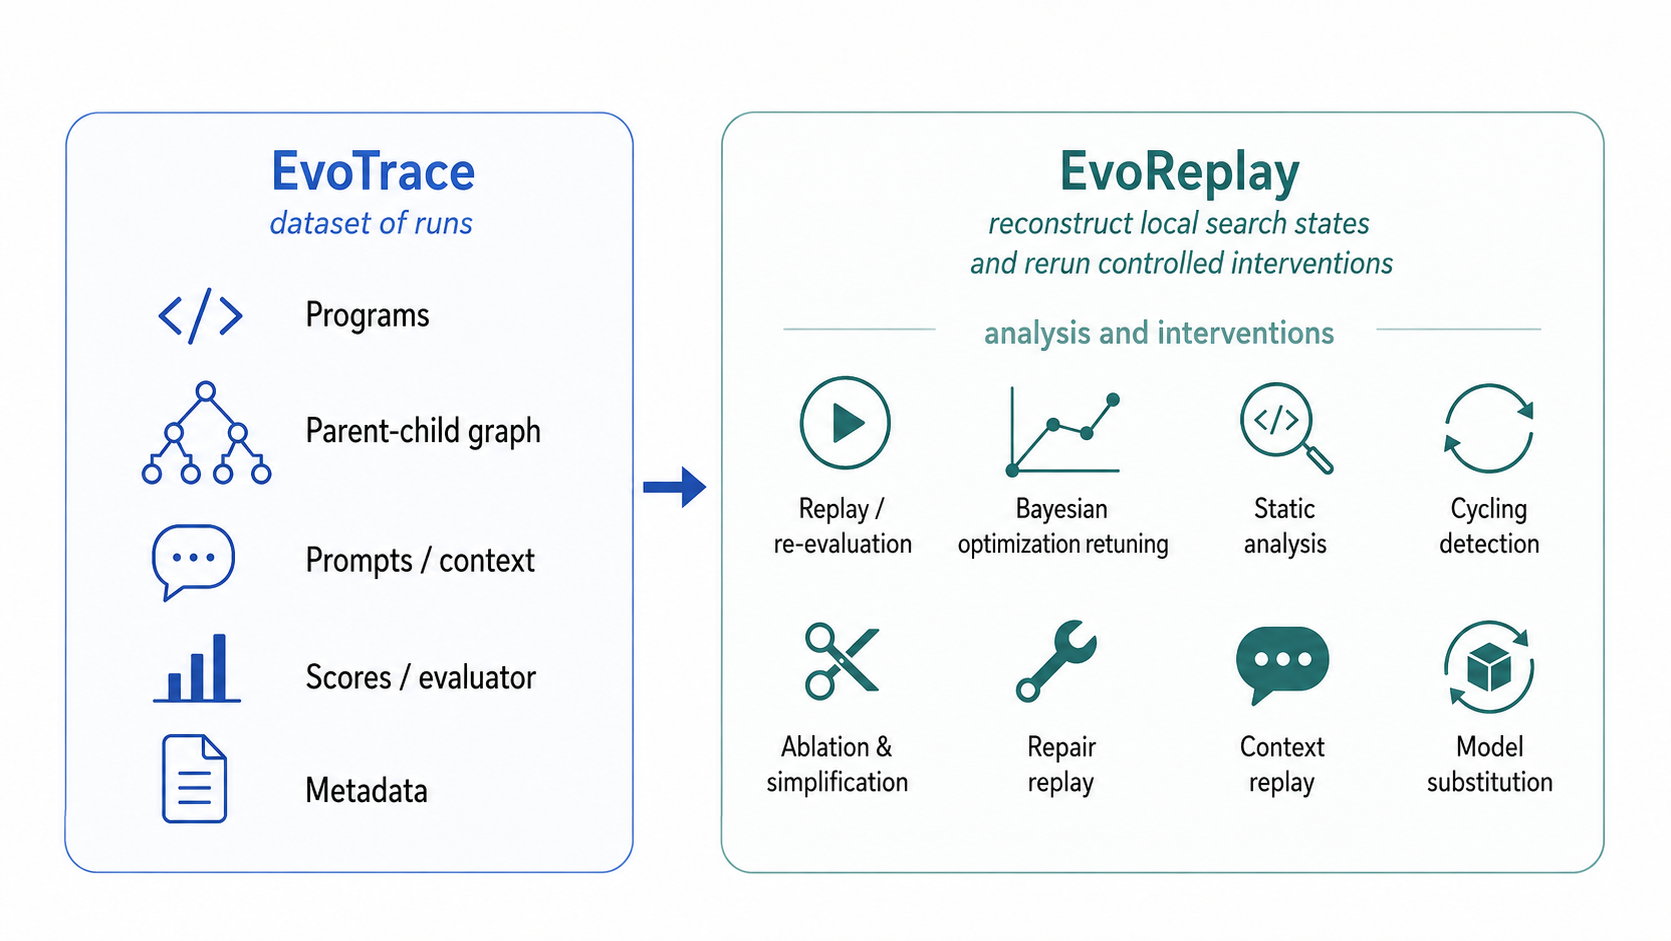
\includegraphics[width=0.65\textwidth]{Figures/main_figure.png}
    \vspace{-1.2em}
    \caption{\textbf{EvoTrace and EvoReplay.} EvoTrace records each evolutionary run as a structured object: programs, parent--child graph, prompts and context, scores, and evaluator metadata. EvoReplay reconstructs local search states from these traces and reruns controlled interventions, including same-prompt replay, Bayesian-optimization retuning, static analysis, cycling detection, ablation, repair, context substitution, and model substitution.}
    \label{fig:overview}
    \vspace{-0.8em}
\end{wrapfigure}replay-based stability tests on score-improving edits (\S\ref{sec:replay}), and a tuning-gap baseline that runs Bayesian optimization over the hyperparameters of a single program (\S\ref{sec:tuning-gap}).

These diagnostics are meant to be practical: the same trace representation and measurements can be integrated into existing open-source evolutionary coding frameworks to reveal whether a run is discovering new algorithmic structure, retuning known patterns, or becoming trapped by its own history. Overall, our results suggest that progress in evolutionary coding is not explained by final scores alone, but depends jointly on the task, the search procedure, the evaluator, and the underlying model family. By measuring the dynamics of search traces, we take a first step toward a systematic understanding of what these agents change over time, which changes matter, and why some runs keep improving while others stall.

\paragraph{Contributions.}
We contribute two artifacts and a set of trace-level findings that use them.
\textbf{(1)~EvoTrace}\footnote{Available at \url{https://huggingface.co/datasets/ZIB-IOL/EvoTrace}.}, a dataset of $121$ evolutionary coding-search runs across four frameworks on $16$ benchmarks spanning Python mathematical constructions and C++ competitive programming problems, with $10{,}672$ unique programs, $18{,}400$ LLM calls, full parent--child graphs, prompts and contexts, scores, and evaluator metadata, normalized into a unified replayable schema (\S\ref{sec:dataset}).
\textbf{(2)~EvoReplay}\footnote{Available at \url{https://github.com/ZIB-IOL/EvoReplay}.}, a methodology and accompanying open-source package that reconstructs local search states from EvoTrace traces and reruns controlled interventions (same-prompt replay, Bayesian-optimization retuning, static analysis, deterministic cycling detection, ablation, repair, and context or model substitution), so that mechanistic claims about a search trajectory can be tested rather than asserted (\S\ref{sec:evoreplay}).
\textbf{(3)~Findings} from applying these tools to characterize how evolutionary coding agents actually behave: which edit types drive score gains, how often runs end up adding back code they had previously deleted (a cycling pattern present throughout the trajectory in nearly all runs), how reliably score-improving programs can be reproduced by re-running the same prompt, how well public scores generalize to held-out evaluation on competitive programming tasks, and how much of a math run's headline gain is recoverable by tuning the hyperparameters of a single mid-run program (\S\ref{sec:experiments}).
